\chapter{Zadatak 4b --- simulacija i paradoks nestabilnosti}
\label{ch:z4-simulacija}

\section{Što se ovdje traži}

Simulirati autonomni sklopni sustav, nacrtati dvije slike --- vremenski odziv i
trajektoriju u prostoru stanja --- i odgovoriti je li sustav stabilan.

\begin{zadatak}{Zadatak 4, podzadatak b)}
b) Simulirajte vremenski promjenjiv sustav (3) s početnim uvjetom
$x(0) = \begin{bsmallmatrix} 1 \\ 0 \end{bsmallmatrix}$, prikažite $x(t)$ (graf
kako se varijable stanja mijenjaju s vremenom) i prikažite trajektoriju sustava u
prostoru stanja. Je li ovaj sustav stabilan?
\end{zadatak}

\begin{predznanje}
\begin{itemize}[nosep,leftmargin=*]
  \item Oba moda su Hurwitzova --- Poglavlje~\ref{ch:z4-hurwitz}.
  \item Razlika vremenskog odziva i faznog portreta --- \S\ref{sec:odziv-fazni}.
  \item Matrična eksponencijala i svojstvene vrijednosti --- \S\ref{sec:svojstvene}.
\end{itemize}
\end{predznanje}

\section{Kako se simulira sustav koji se prespaja}
\label{sec:z4-kako-simulirati}

\begin{korak}[Simulacija po segmentima]
Unutar svakog segmenta $[k,\ k+1)$ matrica dinamike je \emph{konstantna}, pa je
sustav ondje običan LTI sustav i može se integrirati standardnim rješavačem.
Postupak:
\begin{enumerate}[leftmargin=*]
  \item Za $k = 0, 1, \dots, T-1$ odredi parnost od $k$ i odaberi $A_k$.
  \item Integriraj $\dot{x} = A_k x$ na $[k,\ k+1]$ s početnim stanjem $x_k$.
  \item Završno stanje segmenta postaje početno stanje sljedećega:
        $x_{k+1} = x(k+1)$.
\end{enumerate}
Stanje je \emph{neprekidno} u trenucima prespajanja --- skače derivacija, ne
stanje.
\end{korak}

\begin{zamka}[Zamka: integriranje kroz trenutak prespajanja]
Ako se cijeli interval $[0, 20]$ preda \texttt{ode45}-u s funkcijom koja unutar
sebe provjerava parnost $\lfloor t \rfloor$, rješavač će prekoračiti trenutke
prespajanja i adaptivno birati korake preko diskontinuiteta. Rezultat je tiho
netočan --- rješavač pretpostavlja glatku desnu stranu. Ispravno je integrirati
segment po segment, kako je gore, ili barem koristiti \texttt{odeset} s
\texttt{Events}. Ovo je najčešća greška u ovom podzadatku i ne javlja se kao
poruka, nego kao pogrešna slika.
\end{zamka}

\begin{seminar}{Seminar v1.2, §5.3 --- ,,(b) Simulacija sklopnog sustava``}
Autonomni sustav ($u \equiv 0$) simulira se po segmentima duljine $1$ s, jer je
unutar svakog segmenta matrica dinamike konstantna. Na svakom segmentu koristi se
\texttt{ode45}, a završno stanje segmenta postaje početno stanje sljedećeg.

\begin{lstlisting}[style=matlabstyle]
A_par = [-1, -pi/6;   3*pi/2, -1];
A_nep = [-1, -3*pi/2; pi/6,   -1];
x0 = [1; 0];  T = 20;

tt = [];  xx = [];  xc = x0;
for kseg = 0:T-1
    if mod(kseg, 2) == 0, Aa = A_par; else, Aa = A_nep; end
    o = odeset('RelTol', 1e-9, 'AbsTol', 1e-11);
    [ts, xs] = ode45(@(t, x) Aa*x, [kseg, kseg+1], xc, o);
    tt = [tt; ts];  xx = [xx; xs];  xc = xs(end,:)';
end
\end{lstlisting}
\end{seminar}

\section{Slika i njezino čitanje}
\label{sec:z4-slika-otvoreni}

\begin{figure}[H]
\centering
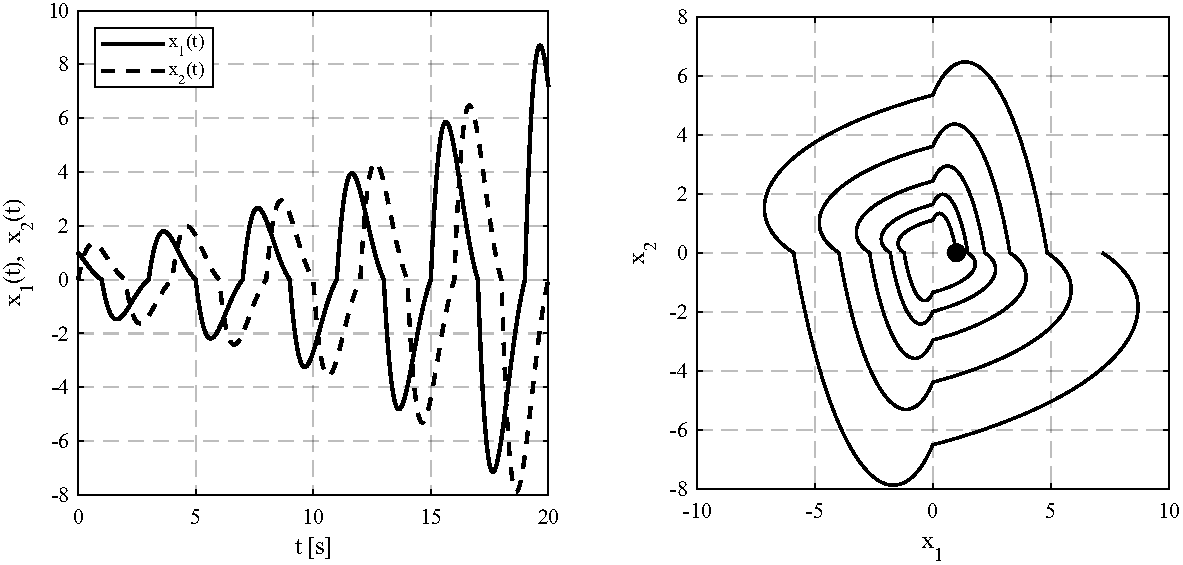
\includegraphics[width=0.95\linewidth]{../figures/fig4_1_open_loop_divergence.pdf}
\caption{Otvoreni krug uz $x(0) = [1,\,0]\trans$: vremenski odziv varijabli stanja
(lijevo) i trajektorija u prostoru stanja (desno). Slika 5.1 seminara v1.2.}
\label{fig:z4-otvoreni}
\end{figure}

\begin{longtable}{@{}p{0.30\linewidth} p{0.66\linewidth}@{}}
\toprule
\textbf{Element} & \textbf{Što je i što pokazuje} \\
\midrule
\endhead
Lijevi graf, os $t$ & Vrijeme $0$ do $20$ s. \\[5pt]
Lijevi graf, puna krivulja & $x_1(t)$; crtkana je $x_2(t)$. Obje osciliraju s
periodom oko $4$ s. \\[5pt]
Omotnica lijevog grafa & \textbf{Raste}. Na početku su amplitude reda $1$, na
kraju prelaze $8$. To je jedini zaključak koji se s tog grafa traži. \\[5pt]
Desni graf & Fazni portret: $x_1$ na apscisi, $x_2$ na ordinati; vrijeme je
sakriveno. \\[5pt]
Puna točka & Početno stanje $x(0) = (1,\,0)$. \\[5pt]
Oblik trajektorije & Spirala koja se \textbf{odmotava} od ishodišta. Zavoji su
uglati --- svakih $90^\circ$ mijenja se mod, pa se mijenja i zakrivljenost. \\
\bottomrule
\end{longtable}

Na kraju simulacije je $\norm{x(20)} = 7{,}19$, sedam puta više nego na početku.
\textbf{Sklopni sustav nije stabilan}, iako su oba moda pojedinačno stabilna.

\begin{zamka}[Zamka: simulacija nije dokaz]
Iz jedne trajektorije, na konačnom vremenu, s jednim početnim uvjetom, strogo
govoreći ne slijedi nestabilnost --- mogla bi to biti duga prijelazna pojava.
Zato seminar dodaje dokaz preko monodromijske matrice. Na obrani reci:
,,simulacija pokazuje rast, a dokaz dajem preko matrice prijelaza stanja preko
jednog perioda``.
\end{zamka}

\section{Dokaz nestabilnosti: monodromijska matrica}
\label{sec:z4-monodromija}

\begin{pojam}{Matrica prijelaza stanja i monodromijska matrica}
Za LTI sustav $\dot{x} = Ax$ rješenje je $x(t) = e^{At}x(0)$, pa je matrica
prijelaza preko jedne sekunde $\Phi = e^{A}$. Za sklopni sustav s periodom
prespajanja $2$ s, matrica koja preslikava $x(2k)$ u $x(2(k+1))$ zove se
\textbf{monodromijska matrica}
\begin{equation}
\Phi_{\mathrm{cikl}} = \Phi_{\mathrm{neparno}}\, \Phi_{\mathrm{parno}} .
\end{equation}
Poredak je bitan: prvo djeluje parni mod, pa neparni --- a matrice se pišu
zdesna nalijevo, kao kompozicija preslikavanja.
\end{pojam}

\begin{korak}[Izračun $e^{A}$ u zatvorenoj formi]
Trik: rastaviti $A$ na skalarni dio i dio koji kvadriranjem daje $-I$.
\begin{enumerate}[leftmargin=*]
  \item \textbf{Rastav.} $A_{\mathrm{parno}} = -I + \frac{\pi}{2}M$, gdje je
        \[
          M = \begin{bmatrix} 0 & -\tfrac13 \\ 3 & 0 \end{bmatrix}.
        \]
        Provjera: $\frac{\pi}{2}M = \begin{bsmallmatrix} 0 & -\pi/6 \\ 3\pi/2 & 0\end{bsmallmatrix}$. \checkmark
  \item \textbf{Ključno svojstvo.}
        $M^2 = \begin{bsmallmatrix} 0 & -1/3 \\ 3 & 0\end{bsmallmatrix}^2
             = \begin{bsmallmatrix} -1 & 0 \\ 0 & -1\end{bsmallmatrix} = -I$.
        Matrica $M$ se, dakle, ponaša kao imaginarna jedinica.
  \item \textbf{Eksponencijala.} Zbog $M^2 = -I$ red za eksponencijalu se
        raspada na parne i neparne članove baš kao kod $e^{j\theta}$:
        \[
          e^{\theta M} = \cos\theta\, I + \sin\theta\, M .
        \]
        Za $\theta = \pi/2$: $\cos\frac{\pi}{2} = 0$, $\sin\frac{\pi}{2} = 1$, pa
        je $e^{\frac{\pi}{2}M} = M$.
  \item \textbf{Spajanje.} Kako $-I$ komutira sa svime,
        \[
          \Phi_{\mathrm{parno}} = e^{A_{\mathrm{parno}}} = e^{-I}e^{\frac{\pi}{2}M}
          = e^{-1} M
          = \begin{bmatrix} 0 & -0{,}122626 \\ 1{,}103638 & 0 \end{bmatrix}.
        \]
\end{enumerate}
\end{korak}

Analogno, uz $A_{\mathrm{neparno}} = -I + \frac{\pi}{2}M'$ i
$M' = \begin{bsmallmatrix} 0 & -3 \\ 1/3 & 0\end{bsmallmatrix}$, $M'^2 = -I$:
\begin{equation}
\Phi_{\mathrm{neparno}} = e^{-1}M' = \begin{bmatrix} 0 & -1{,}103638 \\ 0{,}122626 & 0 \end{bmatrix}.
\end{equation}

\begin{korak}[Monodromijska matrica i spektralni radijus]
\begin{align}
\Phi_{\mathrm{cikl}} &= \Phi_{\mathrm{neparno}}\Phi_{\mathrm{parno}}
= e^{-2} \begin{bmatrix} 0 & -3 \\ \tfrac13 & 0 \end{bmatrix}
         \begin{bmatrix} 0 & -\tfrac13 \\ 3 & 0 \end{bmatrix}
= e^{-2} \begin{bmatrix} -9 & 0 \\ 0 & -\tfrac19 \end{bmatrix} \notag \\
&= \begin{bmatrix} -1{,}218018 & 0 \\ 0 & -0{,}015037 \end{bmatrix}.
\end{align}
Kontrola: $\det \Phi_{\mathrm{cikl}} = e^{-4} = 0{,}018316$, u skladu s
$\det e^{A} = e^{\tr A}$ i $\tr A_{\mathrm{parno}} + \tr A_{\mathrm{neparno}} = -4$. \checkmark

Matrica je dijagonalna, pa su svojstvene vrijednosti dijagonalni elementi:
\begin{formula}{Spektralni radijus}
\begin{equation}
\rho(\Phi_{\mathrm{cikl}}) = \max_i \abs{\lambda_i} = 9e^{-2} = 1{,}218018 > 1 .
\label{eq:z4-rho}
\end{equation}
\end{formula}
Stanje u trenucima $t_k = 2k$ zadovoljava
$x(2(k+1)) = \Phi_{\mathrm{cikl}}\,x(2k)$, dakle
$x(2k) = \Phi_{\mathrm{cikl}}^{\,k}\,x(0)$. Uz $\rho > 1$ norma stanja raste po
geometrijskoj progresiji --- sustav je \textbf{eksponencijalno nestabilan}.
Simulacija je numerička ilustracija tog zaključka.
\end{korak}

\begin{korak}[Odakle zapravo dolazi nestabilnost]
Broj $9$ u $\rho = 9e^{-2}$ objašnjava sve. Svaki mod u jednoj sekundi zakrene
stanje za $90^\circ$ (jer je $\omega = \pi/2$) i priguši ga faktorom
$e^{-1} \approx 0{,}368$. Ali rotacija nije izotropna --- matrice $M$ i $M'$
rastežu jednu os, a stežu drugu, i to \emph{suprotno jedna od druge}:
\begin{align}
M e_1 &= 3\,e_2, & M e_2 &= -\tfrac13\,e_1, \\
M' e_1 &= \tfrac13\,e_2, & M' e_2 &= -3\,e_1 .
\end{align}
Krenemo li od $e_1$, parni mod ga preslika u $3e_2$, a neparni mod baš tu os
rasteže trostruko: $M'(3e_2) = -9e_1$. Zakret od $90^\circ$, dakle, svaki put
dovede stanje točno u onu os u kojoj sljedeći mod ima pojačanje $3$. Dva takva
koraka daju $3 \cdot 3 = 9$, a prigušenje kroz dvije sekunde samo
$e^{-2} \approx 0{,}135$. Kako je $9 \cdot 0{,}135 = 1{,}218 > 1$, rastezanje
pobjeđuje prigušenje.
\end{korak}

\begin{pitanje}{Bi li sustav bio stabilan da se prespaja brže ili sporije?}
\textbf{Odgovor.} Da. Duljina segmenta ulazi u $\Phi = e^{A\tau}$, pa se mijenja
i kut zakreta $\omega\tau$ i prigušenje $e^{-\tau}$. Uz $\tau = 1$ zakret je
točno $90^\circ$ --- najgori mogući slučaj, jer stanje svaki put završi u smjeru
maksimalnog pojačanja sljedećeg moda. Za $\tau$ dovoljno malen ili dovoljno velik
prigušenje pobjeđuje i sustav je stabilan. Zadana jedinična sekunda nije
slučajna: odabrana je tako da paradoks bude što izraženiji.
\end{pitanje}

\begin{ploca}[Kako nacrtati fazni portret otvorenog kruga]
\begin{enumerate}[leftmargin=*]
  \item Osi $x_1$, $x_2$, raspon otprilike $-8$ do $8$.
  \item Označi početnu točku $(1,\,0)$ punom točkom.
  \item Crtaj spiralu koja se \emph{odmotava} u smjeru suprotnom od kazaljke,
        počevši od te točke. Zavoje crtaj uglato, ne glatko --- svakih $90^\circ$
        mijenja se mod.
  \item Nakon pet zavoja izađi izvan okvira i uz zadnji zavoj napiši
        $\norm{x(20)} = 7{,}19$.
  \item Reci naglas: ,,oba su moda stabilna, a sustav divergira; spektralni
        radijus monodromijske matrice je $9e^{-2} = 1{,}218 > 1$``.
\end{enumerate}
\end{ploca}

\begin{izgovor}
,,Sustav sam simulirao po segmentima od jedne sekunde, jer je unutar svakog
segmenta matrica konstantna, pa je sustav ondje LTI. Završno stanje segmenta je
početno stanje sljedećega.

Vremenski odziv pokazuje da amplitude rastu, a fazni portret spiralu koja se
odmotava. Na kraju je norma stanja sedam zarez dva, dakle sedam puta veća nego
na početku. Sklopni sustav dakle nije stabilan --- iako su, kako sam pokazao pod
a), oba moda zasebno Hurwitzova.

Simulacija sama po sebi nije dokaz, pa sam to i dokazao. Matrica prijelaza preko
jedne sekunde je e na a. Zbog rastava a jednako minus i plus pi kroz dva em, gdje
je em na kvadrat jednako minus i, eksponencijala se računa u zatvorenoj formi i
ispada e na minus jedan puta em. Monodromijska matrica preko punog perioda od
dvije sekunde je dijagonalna, s elementima minus devet e na minus dva i minus
jedna devetina e na minus dva. Spektralni radijus je devet e na minus dva, dakle
jedan zarez dva jedan osam, veći od jedan --- norma stanja raste geometrijski.``
\end{izgovor}
